\chapter{Background} \label{Background}
In this chapter I'll introduce the technologies and the phrases that need to be described for proper understanding of my thesis work.
Some of these technologies were only considered during the designing part of the thesis, while others were also present 
during the implementation.

\section{Java} \label{backgrjava}
	Java \cite{java} is a widely-used, object-oriented programming language known for its platform independence, 
	achieved through the Java Virtual Machine (JVM). 

	The backend of Refinery was programmed using the Java programming language. 
	During the thesis, Java is the main programming language being used.

	Java supports object-oriented programming principles like encapsulation, inheritance, and polymorphism, 
	providing code modularity and reusability.
	This comes in handy for the modification of the already existing codebase, while preserving the old implementaiton.

	When working with Java, a Java Development Kit (JDK) has to be installed on the system.
	The Java Development Kit (JDK) is a distribution of Java technology by Oracle Corporation. 
	The Refinery backend project uses JDK 21.

\section{Gradle} \label{backgrgradle}
	Gradle \cite{gradle} is the build automation tool used for the Refinery repository and it greatly helps the package management, 
	building, testing and the local deployment of the project / subprojects.

	Gradle supports Java (section \ref{backgrjava}) as a programming language, which is the language in which the backend of Refinery was written.

	Gradle was designed for multi-project builds, like the Refinery project, consisting of several subprojects. 
	It operates based on a series of build tasks that can run serially or in parallel. 
	This is useful for the backend and the future generator service 
	running simultaneously, locally as separate subprojects.

	Incremental builds and caching of build components are supported, which provide faster build times during the development.

\section{Jetty} \label{backgrjetty}
	Eclipse Jetty \cite{jetty} provides a highly scalable and memory-efficient web server and servlet container, supporting many protocols
	such as HTTP/3,2,1 (section \ref{backgrhttp}) and WebSocket (section \ref{backgrwebsocket}). 
	 
	The original backend of Refinery uses Jetty as its server and could be a viable option for the future generation
	microservice aswell.

\section{JSON} \label{backgrjson}
	JSON (JavaScript Object Notation) \cite{json} is a lightweight data-interchange format. 

	The following description of JSON is by json.org:

	\textit{`JSON is built on two structures:}
	\begin{itemize}
		\item \textit{A collection of name/value pairs. In various languages, this is realized as an object, record, struct, dictionary, hash table, 
		keyed list, or associative array.}
		\item \textit{An ordered list of values. In most languages, this is realized as an array, vector, list, or sequence.'}
	\end{itemize}

	The Refinery web application uses JSON messages as a way to communicate model generation request states
	, results and metadata between the frontend and the backend. It can be a viable communication format for the backend and the 
	future generator microservice.

\section{Hypertext Transfer Protocol} \label{backgrhttp}
	HTTP (Hypertext Transfer Protocol) \cite{httpdoc} is an application layer protocol, 
	designed for enabling communication between clients and servers. 
	HTTP works as a single request - single response protocol between the communicating endpoints.

	HTTP requests are human readable. They consist of the following parts:
	\begin{itemize}
		\item \textbf{Method:} Indicates what type of request the client wants to send to the server. The most used are the following:
		\begin{itemize}
			\item GET requests indicate resource fetching
			\item POST requests indicate resource upload 
			\item PUT / UPDATE requests indicate updating an existing resource
			\item DELETE requests indicate removal of an existing resource
		\end{itemize} 
		\item \textbf{Path:} The path of the resouce for which we send the request 
		\item \textbf{Version:} The version of the HTTP protocol
		\item \textbf{Headers:} Provide additional information for the server that is receiving the request. 
		\item \textbf{Body:} For some requests (e.g.: POST), additional info is provided here.
	\end{itemize}

	The Refinery application utilizes HTTP for both the frontend and the backend of the application. 

\section{REST API} \label{backgrrestapi}
	A REST API \cite{restapi} (also called a RESTful API or RESTful web API) is 
	an application programming interface (API) that conforms to the design principles of 
	the representational state transfer (REST) architectural style. 

	REST API's via the use of the HTTP protocol (section \ref{backgrhttp}) utilize a single request - 
	single response communication methodology.
	REST APIs communicate through HTTP requests to perform standard database functions like creating (POST), reading (GET),
	updating (PUT) and deleting (DELETE) records (also known as CRUD operations) within a resource.

	REST API's can be implemented really easily due to the efforts of many server framework providers. For Java, these include 
	the very popular Spring and Jetty (section \ref{backgrjetty}) frameworks. 

	At the start of the thesis, Refinery does not use or provide any REST APIs, but the implementation of one for the model 
	generation requests could be a viable option.

\section{Remote Procedure Call} \label{backgrpc}
	In distributed computing, a remote procedure call (RPC) \cite{rpc} is when a computer program causes a procedure  
	to execute in a different address space 
	(usually on another computer within the same network), 
	which is written as if it were a local procedure call, without the programmer 
	explicitly writing the details for the remote communication. 
	Via this the programmer writes essentially the same code regardless that the subroutine is local or remote.

	At the start of the thesis, Refinery doesn't use any RPC libraries, however the use of one (like gRPC) could be used for the model generation service implementation.

\section{gRPC} \label{backgrgrpc}
	gRPC (gRPC Remote Procedure Calls) \cite{grpcwiki} is a remote procedure call (RPC) (section \ref{backgrpc}) framework. 
	gRPC uses HTTP/2 for transport.	It generates cross-platform client and server bindings for many languages (which includes 
	Java \ref{backgrjava}). 

	\begin{figure}[h!]
		\begin{center}
			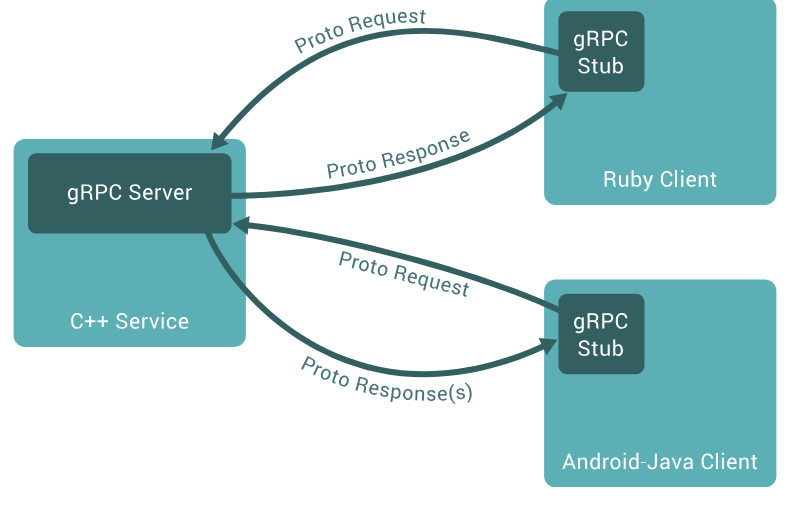
\includegraphics[scale=0.8]{include/imgs/grpc_works.PNG}	
		\end{center}
		\caption{gRPC server and the clients, as represented in gRPC documentation \cite{grpcspec}}
	\end{figure}

	gRPC clients and servers can run and talk to each other in a variety of environments. This includes both on-prem, and more importantly in our case,
	cloud-based environments.

	\subsection{Core concepts}
	Some of the core concepts of gRPC include, but not limited to \cite{grpcspec2}:
	\begin{itemize}
		\item \textbf{Server streaming RPC:} The server responds with multiple responses to the client, which sends a single request. 
		\item \textbf{Deadlines/Timeouts:} gRPC allows clients to specify how long they are willing to wait for an RPC to complete. 
		\item \textbf{Cancelling an RPC:} Either the client or the server can cancel an RPC at any time. 
		A cancellation terminates the RPC immediately.
	\end{itemize}

	The current implementation of Refinery doesn't use the gRPC framework. However, it can be a possible solution for the generator microservice implementaiton. 
	The remote method execution can lower the resource usage of the backend server.

\section{WebSocket} \label{backgrwebsocket}
	The WebSocket Protocol \cite{websocket} enables two-way communication between a client
	and a remote host.
	The goal of
	this technology is to provide a mechanism for applications that need two-way communication with servers that does
	not rely on opening multiple HTTP connections, but using one open connection, for the duration of the communication.

	The following part is taken from RFC 6455 \cite{websocket}, which describes why the creation of WebSocket procotol was needed.

	\textit{
		"Creating web applications using only HTTP, that need bidirectional
		communication between a client and a server has a major problem. 
		It requires the abuse of HTTP to poll the
		server for updates while sending upstream notifications as distinct
		HTTP calls.
		This results in a variety of problems:"
	}
	\begin{enumerate}
		\item \textit{"The server is forced to use a number of different underlying TCP
		connections for each client: one for sending information to the
		client and a new one for each incoming message."}
		\item \textit{"The wire protocol has a high overhead, with each client-to-server
		message having an HTTP header."}
		\item \textit{"The client-side script is forced to maintain a mapping from the
		outgoing connections to the incoming connection to track replies."}
	\end{enumerate}

	\begin{figure}[h!]
		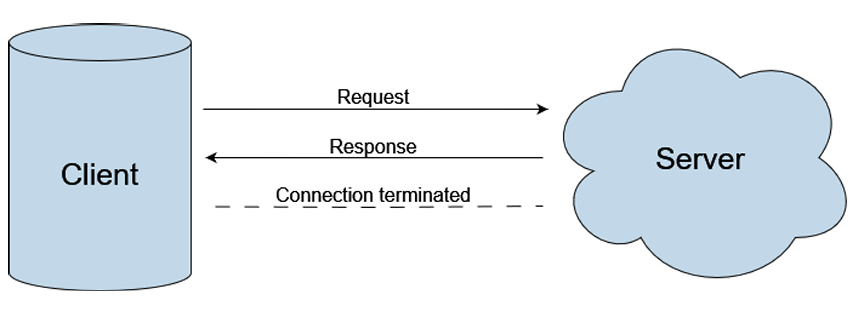
\includegraphics{include/imgs/http.PNG}
		\caption{Regular HTTP connection}
	\end{figure}

	\textit{"A simpler solution would be to use a single TCP connection for
	traffic in both directions. This is what the WebSocket Protocol
	provides. A solution for these HTTP polling scenarios."}

	After the initial WebSocket handshake, the communication protocol is upgraded to WebSocket from HTTP.
	If no communicaiton is happening, the connection is kept alive between the two communicating endpoints via the use of ping and pong messages.
	If a ping sender endpoint doesn't receive a pong response, the connection is lost, and the endpoints are disconnected.
	Other than that, the protocol allows for full bidirectional real-time messaging to the endpoints.

	\begin{figure}[h!]
		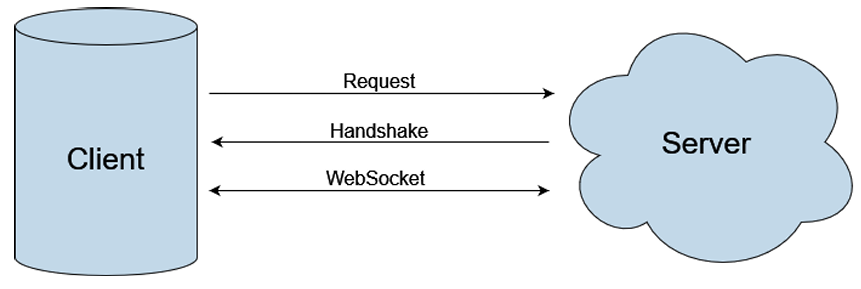
\includegraphics{include/imgs/websocket.PNG}
		\caption{WebSocket connection over HTTP}
	\end{figure}

	The current implementation of Refinery does already utilize WebSocket. The frontend communicates editor changes, model generation
	states, results and metadata via the use of WebSocket. 
	For the implementation of the generator microservice, it could also be a viable solution.

\section{Shell} \label{backgrshell}
	In computing, a shell \cite{shell} is a computer program that exposes an operating system's services to a human user or other programs. 

	In addition to shells running on local systems, there are different ways to make remote 
	systems available to local users; such approaches are usually referred to as remote access (like the use of SSH) or remote administration.

	Within the Refinery project, the use of a CLI based Unix shell (like bash) is needed for the execution of shell scripts. Furthermore, it can come in handy 
	as a remote access for our VMs via the use of SSH, which allows debugging our infrastructure.

\section{Shell script} \label{backgrshellscript}
	A shell script \cite{shellscript} is a computer program designed to be run by a Unix shell (section \ref{backgrshell}). 
	Typical operations performed by shell scripts are file manipulation, program execution.
	The term is also used for the automated mode of running an operating system shell.

	The Refinery project has Unix shell scripts, which automate the build process and the containerization of the application.

\section{Cloud Computing} \label{backgrcloud}
	The following description is taken from a popular public cloud provider's, Google's cloud computing introduction:

	\textit{`Cloud computing \cite{cloud} is the on-demand availability of computing resources (such as storage and infrastructure), as services over the internet. 
	It eliminates the need for individuals and businesses to self-manage physical resources themselves, and only pay for what they use.'}

	\textit{`Cloud computing service models are based on the concept of sharing on-demand computing resources, software, and information over the internet. 
	Companies or individuals pay to access a virtual pool of shared resources, including compute, storage, and networking services, which are located on
	remote servers that are owned and managed by service providers.'}

	The infrastructure of Refinery is described as a public cloud deployment. 
	This means, that the infrastructure is run by third-party cloud service providers.
	The providers offer compute, storage and network resources over the internet. 

	The cloud services used for the deployment of Refinery are called `Infrastructure as a service (IaaS)'.
	IaaS service means \textit{`on-demand access to IT infrastructure services, 
		including compute, storage, networking, and virtualization. It provides the highest level of control over the IT 
		resources and most closely resembles traditional on-premises IT resources.' \cite{cloud} }

	\subsection{Cloud Native} \label{backgrcloudnative}
		This following definition of Cloud Native is taken from AWS's website \cite{cloudnative}:

		\textit{
			`Cloud native is the software approach of building, deploying, and managing modern applications 
			in cloud computing environments. Modern companies want to build highly scalable, flexible, and 
			resilient applications that they can update quickly to meet customer demands. 
			To do so, they use modern tools and techniques that inherently support application
			development on cloud infrastructure. These cloud-native technologies support fast 
			and frequent changes to applications without impacting service delivery, providing
			adopters with an innovative, competitive advantage.'
		}

		The implementation of the Refinery web application is a cloud native application. It is deployed 
		and managed in the AWS cloud (section \ref{backgraws}).

	\subsection{Scaling} \label{backgrscaling}
		The following explanation of scaling is taken from VMWare's website \cite{scaling}:

		\textit{
			`Scaling  in cloud computing refers to the ability to increase or decrease IT resources as
			needed to meet changing demand. Scalability is one of the hallmarks of the cloud and the primary driver 
			of its exploding popularity with businesses. Scaling allows the businesses to pay only for the resources that
			they truly need.
			\begin{itemize}
				\item \textbf{Vertical scaling:} (also referred to as “scaling up” or “scaling down”) 
				You add or subtract power to an existing cloud server upgrading memory (RAM),
				storage or processing power (CPU).
				Usually this means that the scaling has an upper limit based on the capacity of the server
				or machine being scaled; scaling beyond that often requires downtime.
				\item \textbf{Horizontal scaling:} (also referred to as "scaling in" or "scaling out"), 
				You add more resources like servers to your system to spread out the workload across machines, 
				which in turn increases performance and storage capacity. 
				Horizontal scaling is especially important for businesses with high availability services requiring 
				minimal downtime.'
			\end{itemize}
		}
		The deployment of Refinery's infrastructure utilizes scaling via the use of application 
		auto scaling (section \ref{backgautoscaling}).

	\subsection{Load Balancing} \label{backgrloadbalance}
		The following parts regarding load balancing are taken from Cloudflare \cite{loadbalancing}:

		\textit{
			`Load balancing \cite{loadbalancing} is the practice of distributing computational workloads between two or more computers. 
			On the Internet, load balancing is often used for dividing network traffic among several servers. 
			This reduces the strain on each server and makes the servers more efficient, speeding up performance and 
			reducing latency.  
			By dividing user requests among multiple servers, user wait time is vastly reduced. 
			This results in a better user experience.'
		}

		\textit{
			`Load balancing is handled by a tool or application called the load balancer. A load balancer can be 
			either hardware-based or software-based. 
			Load balancers determine which server should handle each request 
			based on a number of different algorithms. 
			These algorithms fall into two main categories: static and dynamic.'
		}
		\begin{itemize}
			\item \textit{\textbf{Static load balancing} algorithms distribute workloads without taking into account the current 
			state of the system. }
			
			\item \textit{\textbf{Dynamic load balancing} algorithms take the current availability, workload, 
			and health of each server into account. 
			}
		\end{itemize}

		The deployment of Refinery's infrastructure utilizes load balancing. The balancing algorithm can be round-robin (static) and 
		least connection (dynamic), as AWS load balancers (section \ref{awslb}) provide these algorithms from the start.

\section{Amazon-related cloud technologies}
	\subsection{Amazon Web Services(AWS)} \label{backgraws}
		Amazon Web Services (AWS) \cite{aws} is the public cloud offerring by Amazon. AWS has a vast offering
		of services, which help its end-users manage the infrastructures needed to host their own applications.
		AWS services are delivered to customers via a network of AWS server farms located throughout the world.

		The project uses Amazon Web Services for the infrastructure of Refinery. 
		It should be deployed in the Stockholm region.

		In the following sections (2.14.2 - 2.14.6), I will go into detail what some of those services are and how
		they can be beneficial for the users of those services.

	\subsection{Amazon Elastic Compute Cloud (EC2)} \label{backgrec2}
		Amazon Elastic Compute Cloud (Amazon EC2) \cite{ec2} provides on-demand, scalable computing capacity in the Amazon 
		Web Services (AWS) Cloud.  
		Amazon EC2 instances are virtual machine (VM) instances running in Amazon's cloud environment (AWS). 
		The amount of VMs can be scaled based on resource usage via the use of auto scaling (section \ref{backgautoscaling}).

		The Refinery web application can be deployed on running EC2 instances.

	\subsection{Amazon Elastic Container Service (ECS)} \label{backgecs}
		Amazon Elastic Container Service (Amazon ECS) \cite{ecs} is a fully managed container orchestration service that helps 
		the deployment, management, and scaling of containerized (section \ref{backgcontainer}) applications. 
		It is integrated with both AWS and third-party tools, 
		such as the Docker and GitHub registry. This integration makes the deployment of Refinery easier.

		There are three main layers of Amazon ECS \cite{ecs}:
		\begin{enumerate}
			\item \textit{\textbf{Capacity:} The infrastructure where the users run their containers. Options include Amazon EC2, 
			AWS Fargate and On-prem virtual machines and servers (infrastructure outside of Amazon) }
			\item \textit{\textbf{Controller:} The deployment and management of the applications that are run on the containers. The Amazon
			ECS scheduler is the software that manages / controls the applications.}
			\item \textit{\textbf{Provisioning:} The tools used for interfacing with the ECS scheduler to deploy and manage the applications.
			and containers. Options include the AWS Management Console (Web GUI), AWS Command Line Interface (CLI), 
			AWS Software Development Kits (SDKs).}
		\end{enumerate}

		Amazaon ECS can be a valid option for the provisioning of Refinery's services. The AWS Management Console 
		can be used for provisioning.

	\subsection{Virtual Private Cloud (VPC)} \label{backgvpc}
		The following introduction is from Amazon's documentation \cite{vpc}:

		\textit{`With Amazon Virtual Private Cloud (Amazon VPC) \cite{vpc}, users can launch AWS resources in a logically 
		isolated virtual network that is defined by the user. This virtual network closely resembles a traditional network 
		that the user would operate, with the benefits of using the scalable infrastructure of AWS.'}

		The deployment of Refinery's infrastructure is done within one Virtual Private Cloud. This way even if 
		the application instances are running on a different subregion of Amazon's cloud, they are connected within one network.

	\subsection{Elastic Load Balancing (ELB)} \label{backgelb}
		The following introduction is from Amazon's documentation \cite{elb}:

		\textit{`Elastic Load Balancing \cite{elb} automatically distributes incoming traffic across multiple targets, 
		such as EC2 instances, containers, and IP addresses. 
		It monitors the health of its registered targets, and routes traffic only to the healthy targets. 
		Elastic Load Balancing scales load balancers as the incoming traffic changes over time.'}

		Elastic Load Balancing supports the following load balancers: 
		\begin{itemize}
			\item Application Load Balancers
			\item Network Load Balancers
			\item Gateway Load Balancers
			\item Classic Load Balancers
		\end{itemize}

		\subsubsection{Application Load Balancer} \label{backgalb}
			The following introduction is from Amazon's documentation \cite{elb}:

			\textit{`An Application Load Balancer \cite{elb} functions at the application layer, the seventh layer of the Open Systems Interconnection (OSI)
			model. After the load balancer receives a request, it evaluates the listener rules in priority order to determine which 
			rule to apply, and then selects a target from the target group for the rule action. 
			Routing algorithm can be configured at the target group level. 
			The default routing algorithm is round robin; alternatively, the least outstanding requests routing algorithm can be used aswell.'}

			\textit{`Health checks can be configured, which are used to monitor the health of the registered targets so that the 
			load balancer can send requests only to the healthy targets within a target group.'}

			The application load balancer can be utilized for the Refinery applications. This allows our scaling services (like the backend and 
			the generator) to receive requests based on the set load balancing algorithm. The services should be setup as separate target groups.

	\subsection{Application Auto Scaling} \label{backgautoscaling}
		The following introduction is from Amazon's documentation \cite{autoscale}:
		\textit{`Application Auto Scaling \cite{autoscale} is a web service for automatically scaling scalable resources 
		for individual AWS services beyond Amazon EC2. Application Auto Scaling allows automatic scaling of 
		scalable resources according to conditions that are defined.'}

		The auto scaling is useful for the scaling of containerized Refinery services (backend, and generator service).

\section{Containers} \label{backgcontainer}
	The following introduction for containers is taken from RedHat's website \cite{container}:
	\textit{
	`Containerization \cite{container} is the packaging together of software code with all it’s necessary 
	components like 
	libraries, frameworks, and other dependencies so that they are isolated in their own container.'}
	
	\textit{`This is done so that the software or application within the container can be moved and run consistently 
	in any environment and on any infrastructure, independent of that environment or infrastructure’s 
	operating system. It is a fully functional 
	and portable computing environment.'}

	\textit{`Containers are often used to package single functions that perform specific tasks—known as a microservice. 
	Microservices are the breaking up of the parts of an application into smaller, more specialized services.'}

	The services of the Refinery application should be developed with containerization in mind. This makes 
	the distribution and deployment of the application much easier.

	\subsection{Docker} \label{backgdocker}
		According to Docker's documentation \cite{docker}:

		\textit{
			`Docker \cite{docker} is an open platform for developing, shipping, and running applications. 
			Docker provides the ability to package and run an application in a loosely isolated environment 
			called a container. The isolation and security lets you run many containers simultaneously 
			on a given host.'
		}

		\textit{
			`Docker containers can be created by running docker images. Images are templates 
			containing the read-only instructions needed 
			to create the container running our application. To build an image, the user has to write a Dockerfile
			where they specify all of the steps needed to build their image (like linking libraries, exposing ports, 
			setting environment variables, etc.')
		}

		\textit{
			`The docker container is the running instance of the docker image. Those can be run by the use of the docker cli.'
		}

		The implemented Refinery services can be containerized via the use of Docker images. The images can be uploaded to the 
		Docker Registry, providing easier distribution.


	\subsection{Docker Compose} \label{backgdockercompose}
		According to Docker \cite{dockercompose}:

		\textit{
			`Docker Compose \cite{dockercompose} is a tool for defining and running multi-container applications. 
			It is the key to unlocking a streamlined and efficient development and deployment experience.'
		}

		\textit{
			Compose simplifies the control of the entire application stack, making it easy to manage services, 
			networks, and volumes in a single, comprehensible YAML configuration file. 
			With a command, all of the services from the configuration file can be started.
		}

		Within the scope of the thesis, Docker Compose can be used for the local deployment of 
		the containerized Refinery backend and generator services. This provides manual testing abilities
		before deploying the application on the cloud.

